\documentclass[10pt,letterpaper]{article}
\usepackage[T1]{fontenc}
\usepackage{times,microtype,graphicx,booktabs,float}
\usepackage[font=small,labelfont=bf,labelsep=period,skip=4pt]{caption}
\setlength{\textwidth}{6in}
\setlength{\textheight}{9in}
\setlength{\oddsidemargin}{0.25in}
\setlength{\evensidemargin}{0.25in}
\setlength{\topmargin}{-0.35in}
\setlength{\headheight}{0.15in}
\setlength{\headsep}{0.2in}
\setlength{\parindent}{0pt}
\setlength{\parskip}{4pt}
\setlength{\intextsep}{4pt}
\setlength{\textfloatsep}{9pt}
\newcommand{\reporttitle}[2]{\noindent\rule{\linewidth}{4pt}\par
{\LARGE\bfseries #1\par}\vspace{2pt}\noindent\rule{\linewidth}{1pt}\par
#2\par October 16, 2026\par\vspace{4pt}}
\makeatletter
\renewcommand\section{\@startsection{section}{1}{\z@}{9pt}{4pt}{\large\bfseries}}
\makeatother
\renewenvironment{abstract}{\small\textbf{Abstract}\par}{\par\vspace{3pt}}
\let\originalitemize\itemize
\renewcommand{\itemize}{\originalitemize\setlength{\itemsep}{1pt}\setlength{\parskip}{0pt}\setlength{\parsep}{0pt}}
\let\originalenumerate\enumerate
\renewcommand{\enumerate}{\originalenumerate\setlength{\itemsep}{1pt}\setlength{\parskip}{0pt}\setlength{\parsep}{0pt}}
\begin{document}
\reporttitle{Adapter trimming comparison}{Two Arabidopsis bulk ATAC biological replicates; paired input}
\begin{abstract}At 1 million pairs, untrimmed input retains 458,813 and 565,032 eligible fragments. Cutadapt and fastp alter these totals by at most 62 fragments each, and peak Jaccard remains above 0.9995. The inspected archived reads are only 31 bases long, limiting generalization to longer libraries. We would retain explicit protocol-specific trimming decisions.\end{abstract}
\section*{Setup}
\textbf{Data.} SRR4000468 and SRR4000469 are biological replicates from seven-day Arabidopsis seedlings. The archived first 100 records per mate are 31 bases long; this is an inspection result, not a full-library length census.

\textbf{Comparisons.} No trimming, Cutadapt 5.2 and fastp 1.4.0 use the explicit Nextera adapter CTGTCTCTTATACACATCT, with unrelated fastp filters disabled. All arms keep the same reference, alignment, duplicate policy and MACS3 settings.

\textbf{Scoring.} Retention is eligible nuclear fragments divided by raw input pairs, not the fraction exiting the trimmer. Peak Jaccard is base-pair intersection/union; fixed-region Spearman uses identical baseline regions. Output-pair retention from trimming alone is not inferred from downstream retention.

\begin{table}[H]\centering\small\caption{Input identities at the atac-arabidopsis-1m cap.}
\begin{tabular}{lrr}\toprule
Library & Role / control & Raw templates \\ \midrule
SRR4000468 & biological replicate 1 & 1,000,000 \\
SRR4000469 & biological replicate 2 & 1,000,000 \\
\bottomrule\end{tabular}\end{table}
\section{Trimming produces small changes in these short-read libraries}
The 2 Cutadapt fixed-region correlations exceed 0.99998. Fastp reports 4,995 and 3,042 peaks, compared with 4,997 and 3,043 for untrimmed input.

\begin{figure}[H]\centering\makebox[\linewidth][c]{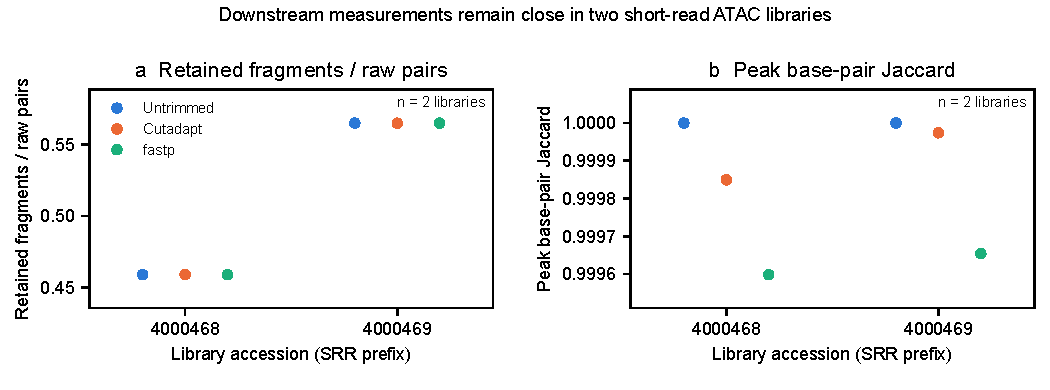
\includegraphics[width=7in]{figures/trimming-quality.pdf}}
\caption{Downstream fragment retention and peak-base agreement.}\end{figure}
\newpage
\section{The processing times are close on this cohort}
Across 3 fresh technical repetitions per arm, cohort timing includes both biological libraries and subsequent processing. These are 14-CPU-budget runs; they do not isolate trimmer execution time or establish a throughput ranking for long reads.

\begin{figure}[H]\centering\makebox[\linewidth][c]{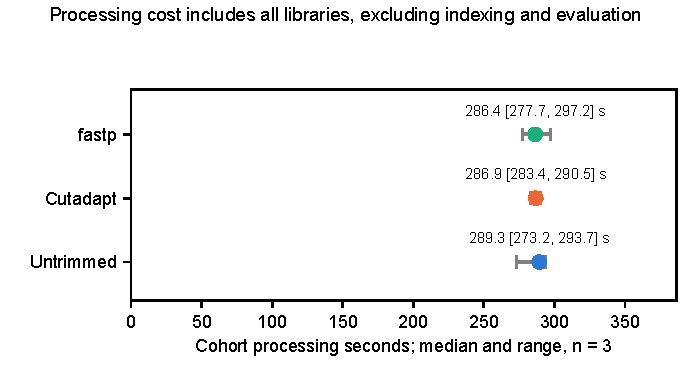
\includegraphics[width=4.6in]{figures/trimming-cost.pdf}}
\caption{Cohort wall time by trimming policy; ranges are observed.}\end{figure}
\begin{table}[H]\centering\small\caption{Recorded median measurements; nd means not determined.}
\begin{tabular}{lrr}\toprule
Method & Library & Spearman \\ \midrule
baseline & SRR4000468 & 1.000000 \\
baseline & SRR4000469 & 1.000000 \\
cutadapt & SRR4000468 & 0.999980 \\
cutadapt & SRR4000469 & 0.999988 \\
fastp & SRR4000468 & 0.999980 \\
fastp & SRR4000469 & 0.999986 \\
\bottomrule\end{tabular}\end{table}
\section*{Open issues}
\begin{itemize}
\item The first-100-read inspection cannot prove that every read is adapter-free.
\item Long-read and adapter-rich libraries need separate comparisons.
\item Standalone trimming pair-loss and phase-specific speed are not inferred from downstream totals.
\end{itemize}
\section*{Recommendation}
We would defer a universal trimming change and retain declared adapter policies.

\begin{enumerate}
\item Compare longer paired reads with measured adapter burden.
\item Report trimmer output pairs separately from alignment and fragment selection.
\end{enumerate}
\section*{Appendix: Methods}
We summarize recorded results without rerunning biological processing. The main Arabidopsis matrix uses seeded nested raw-template subsets (seed 60141), three fresh technical repetitions at the 1-million cap and one at the 5-million cap. Actual counts replace requested caps for short libraries. DAP retains primary mapped reads including MAPQ 0; ATAC selects proper primary pairs with both mates MAPQ at least 30, excludes MAPQ 255, organelles and marked duplicates. Biological identity is preserved. Source files are SHA-256 checked against the accompanying catalog; evidence snapshot revision ed1c50b8e4b5 includes the October 13 to 16 records. Completed local reference assessments are separately identified in that catalog.

\end{document}
